\begin{figure}[H]
    \centering
    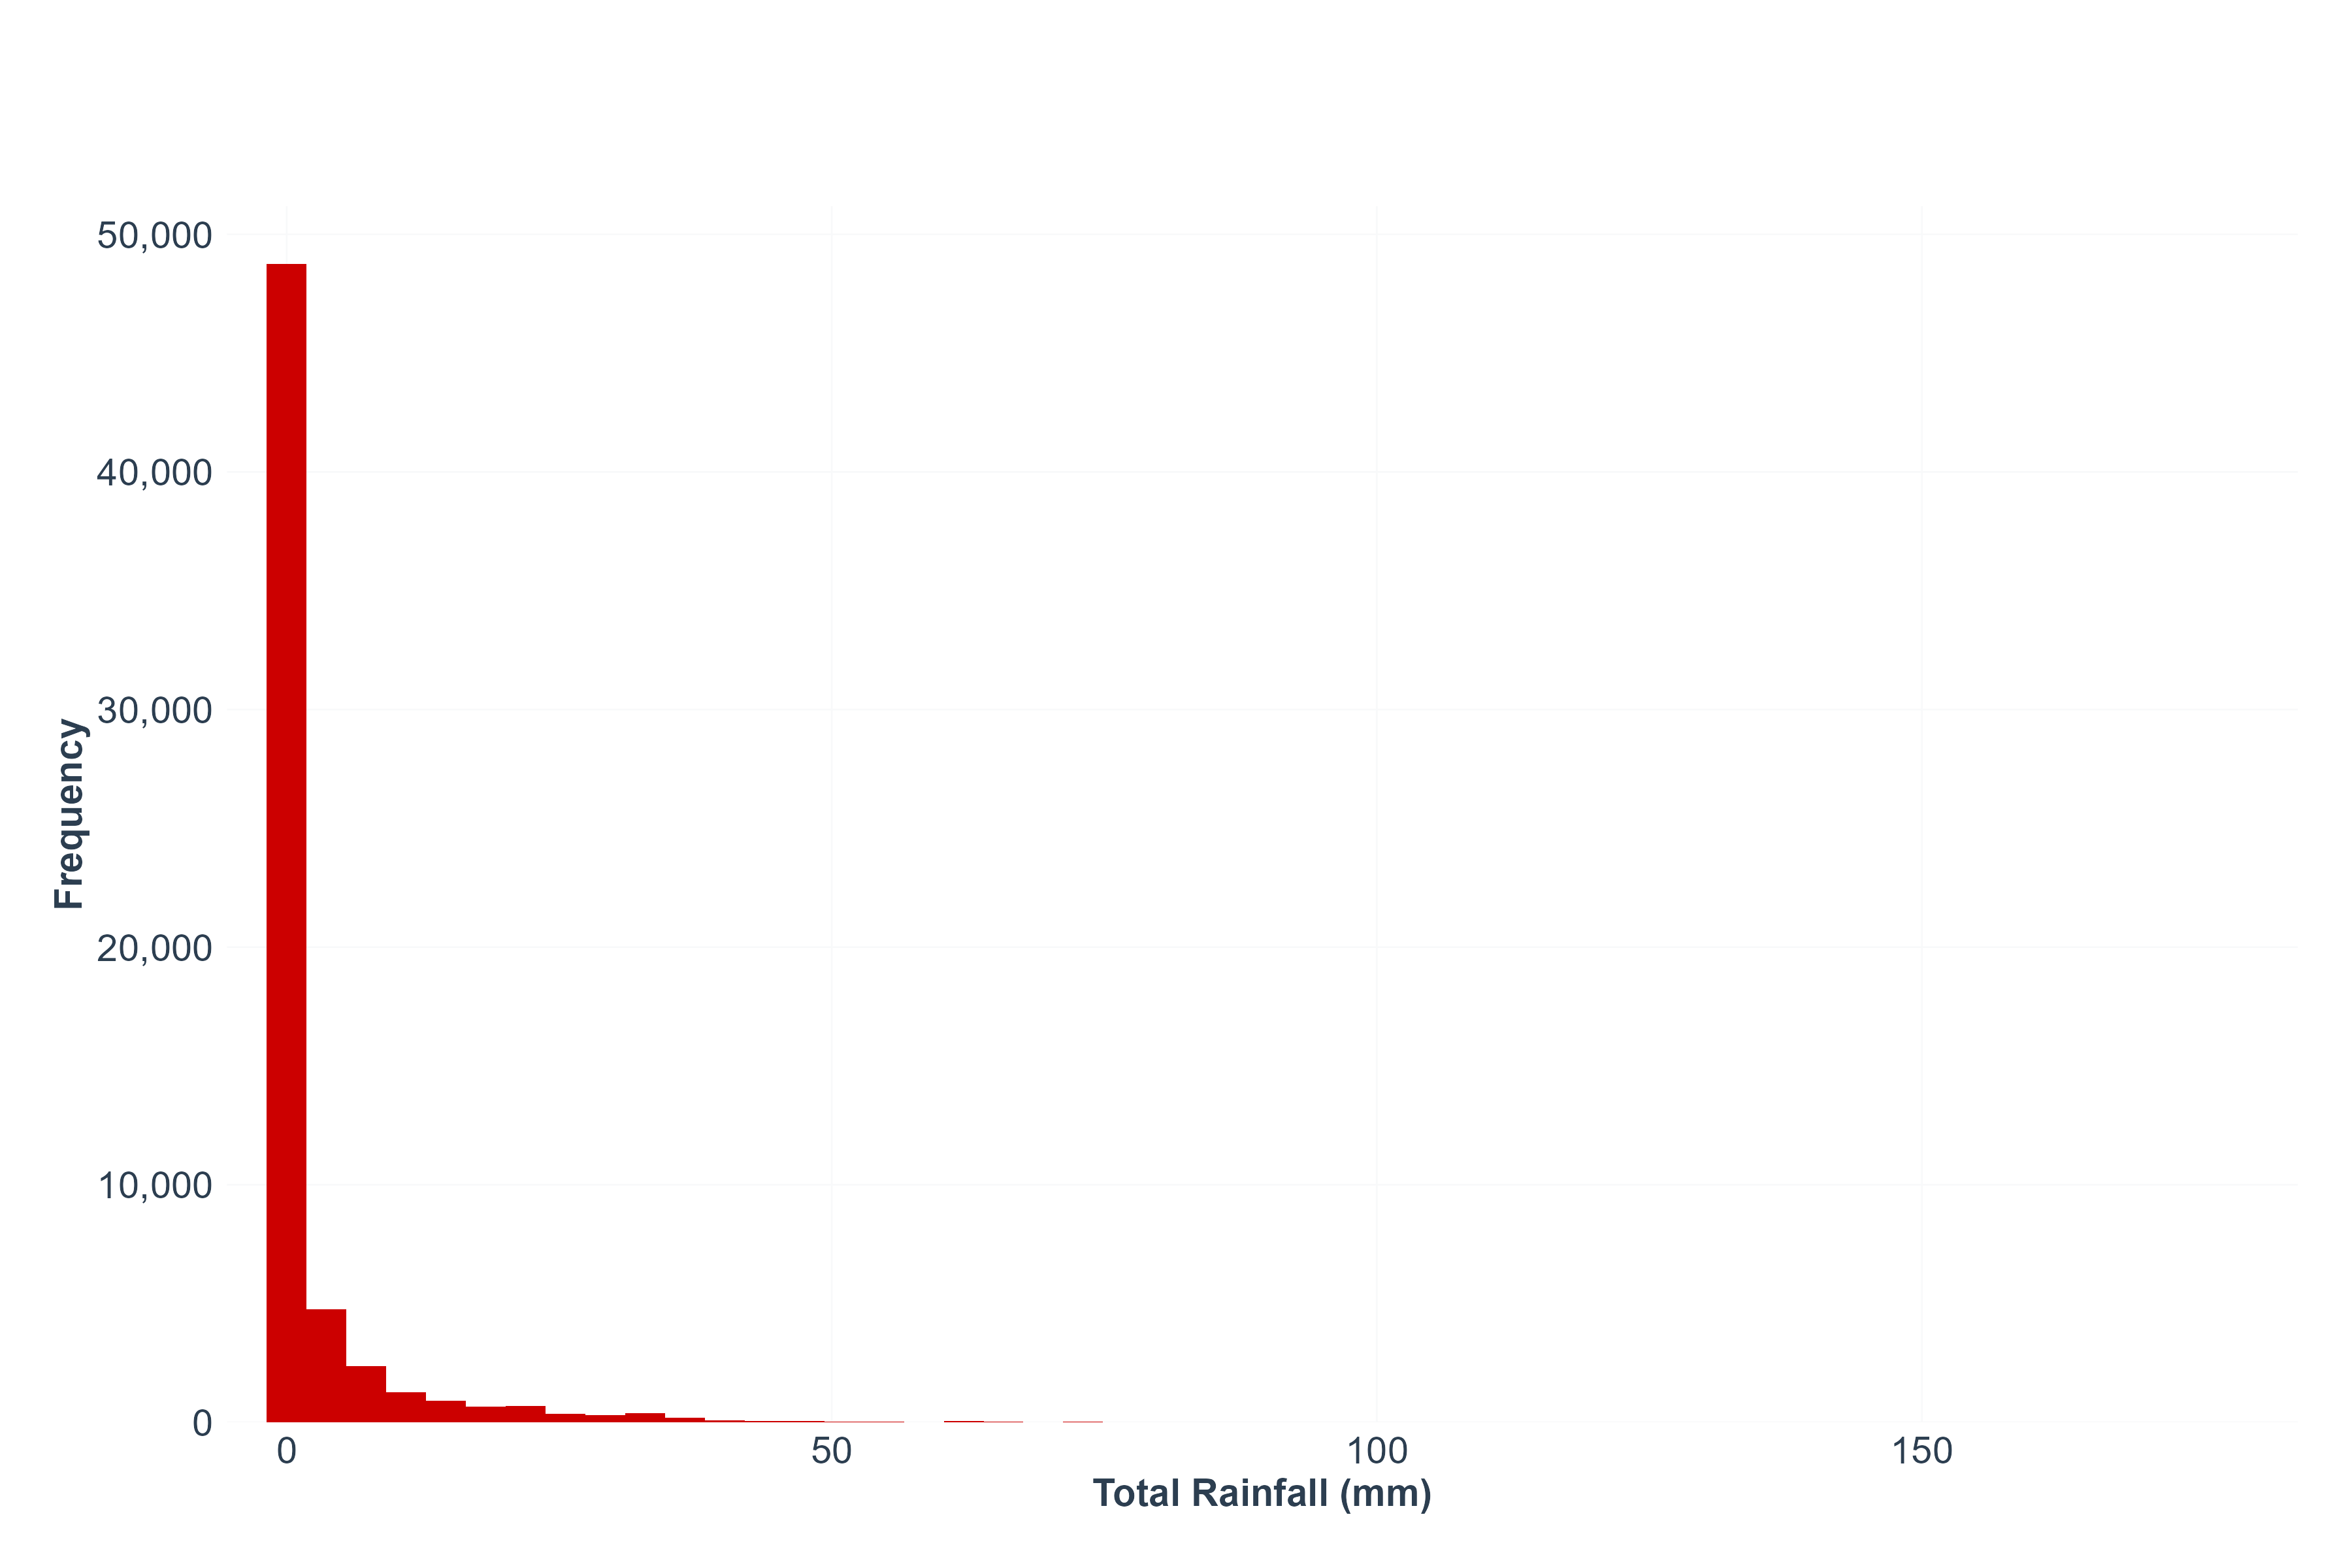
\includegraphics[width=0.8\textwidth]{../figures/rainfall_histogram.png}
    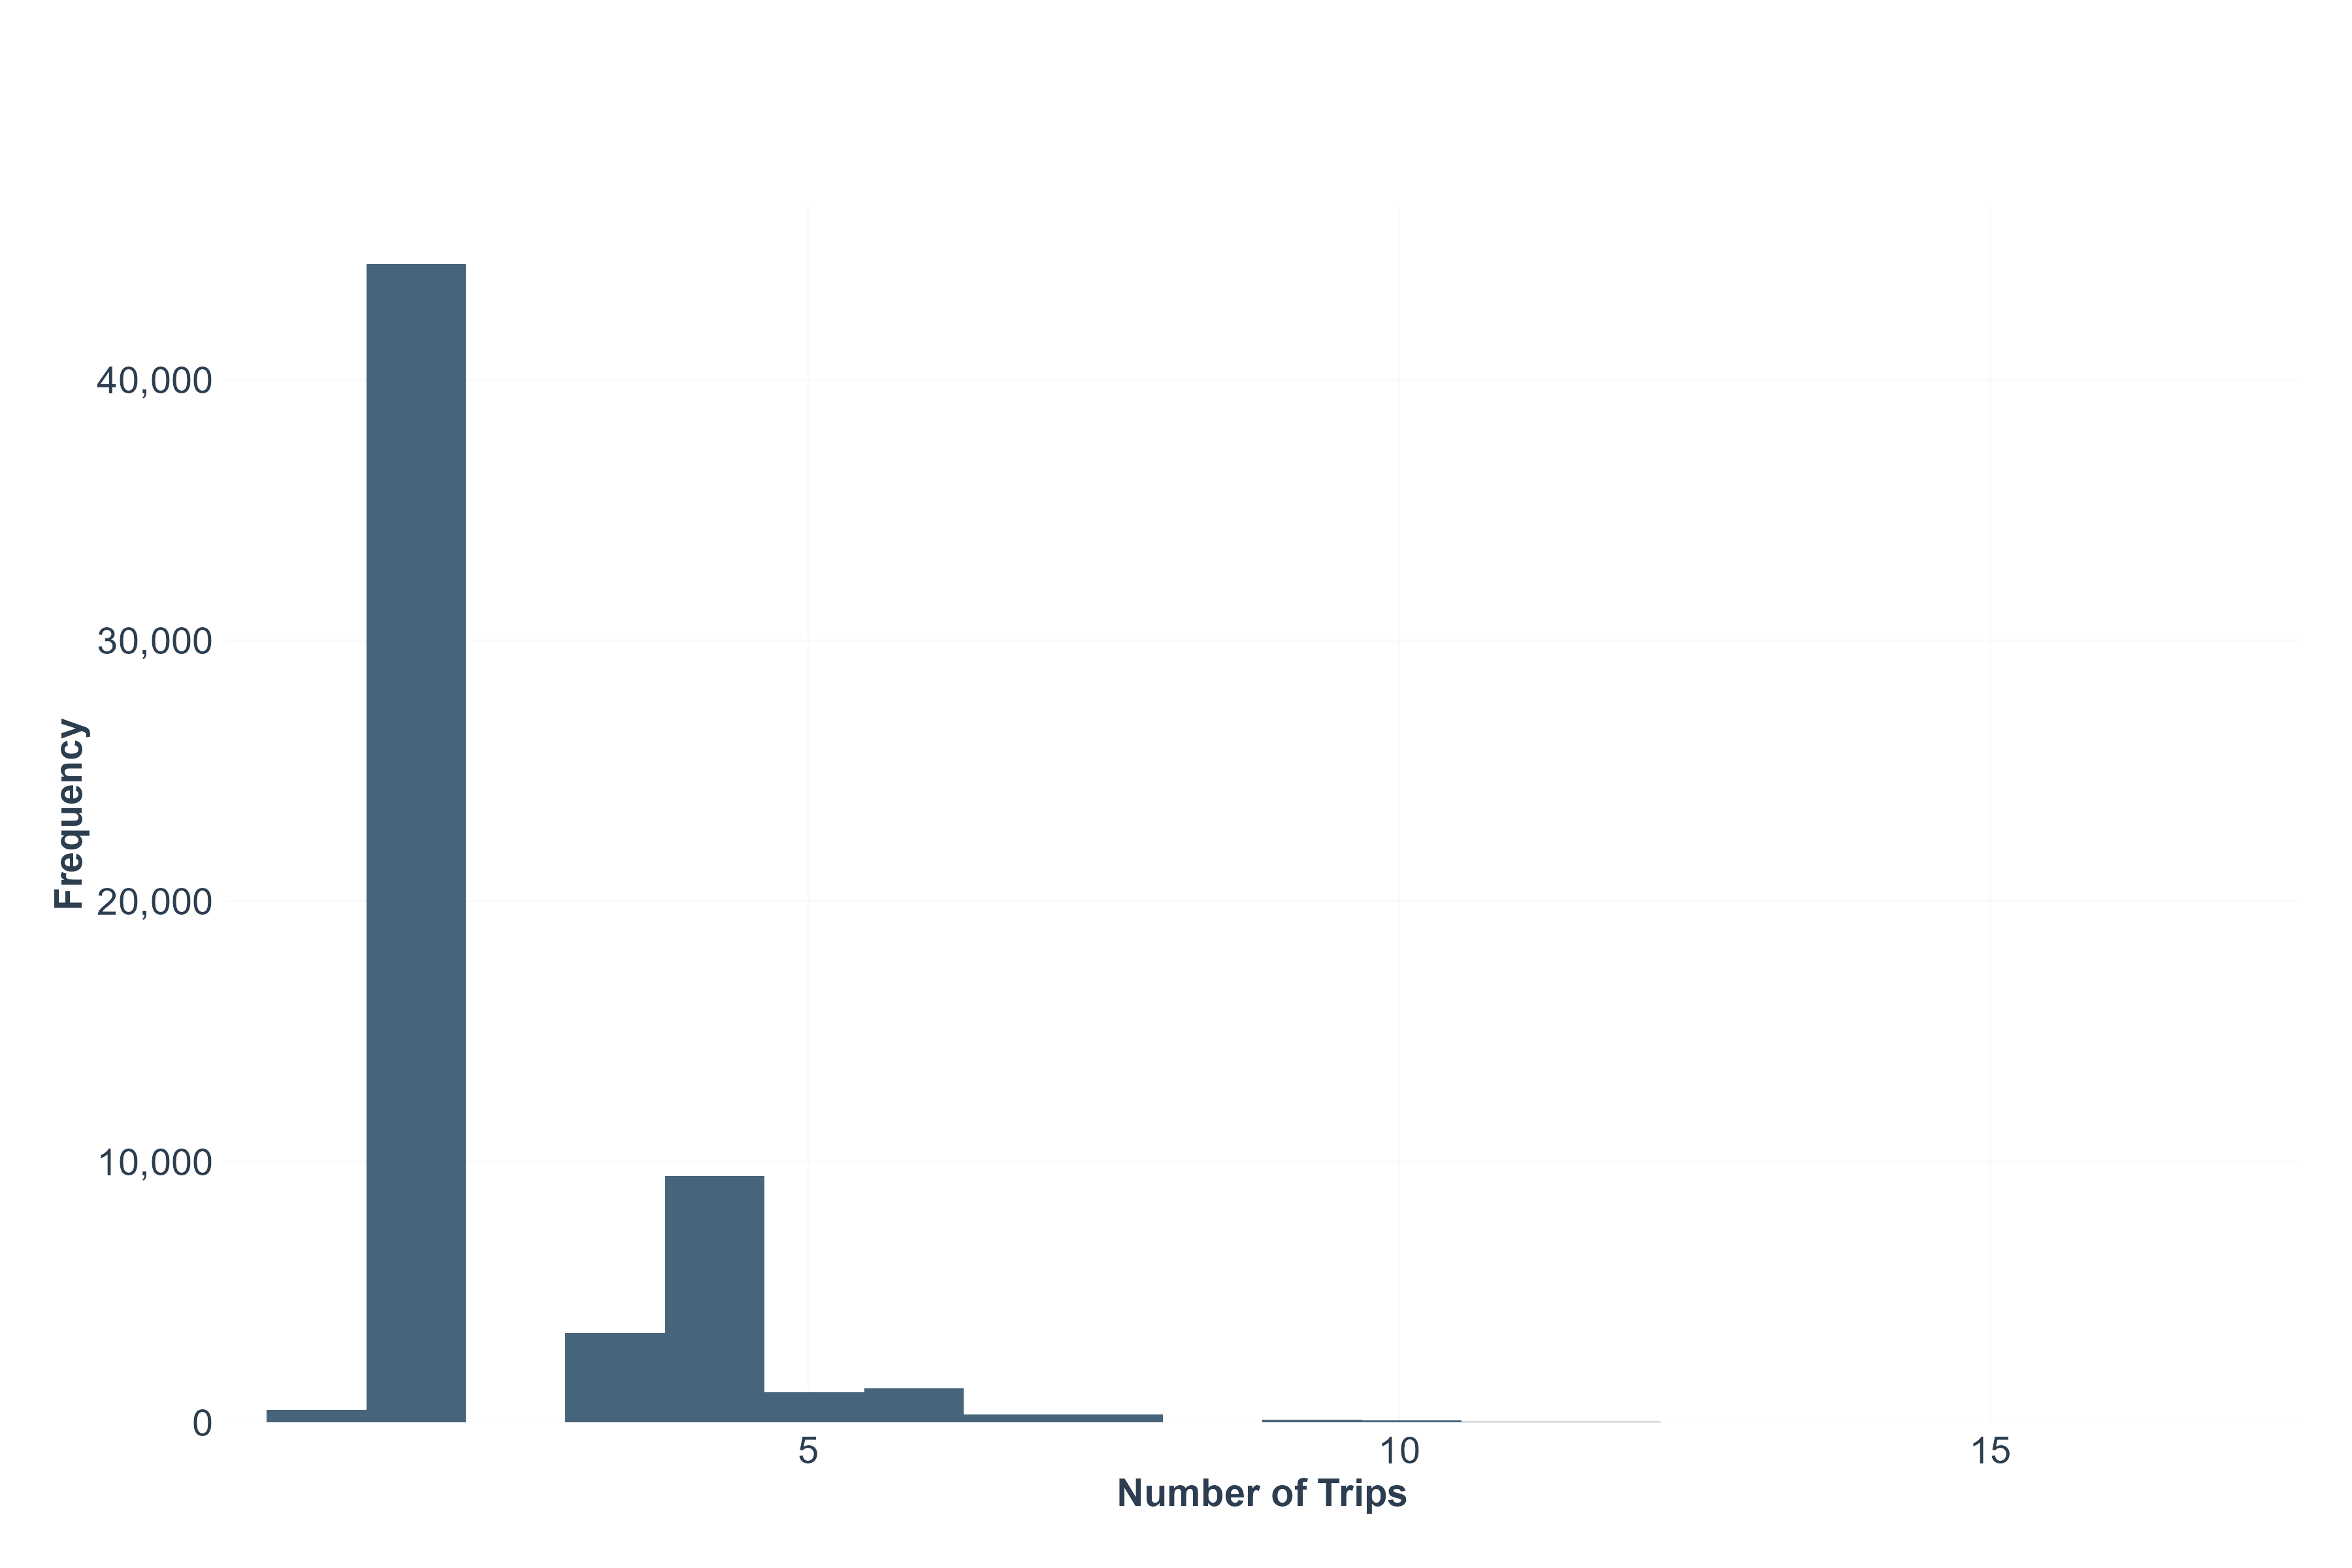
\includegraphics[width=0.8\textwidth]{../figures/trips_histogram.png}
    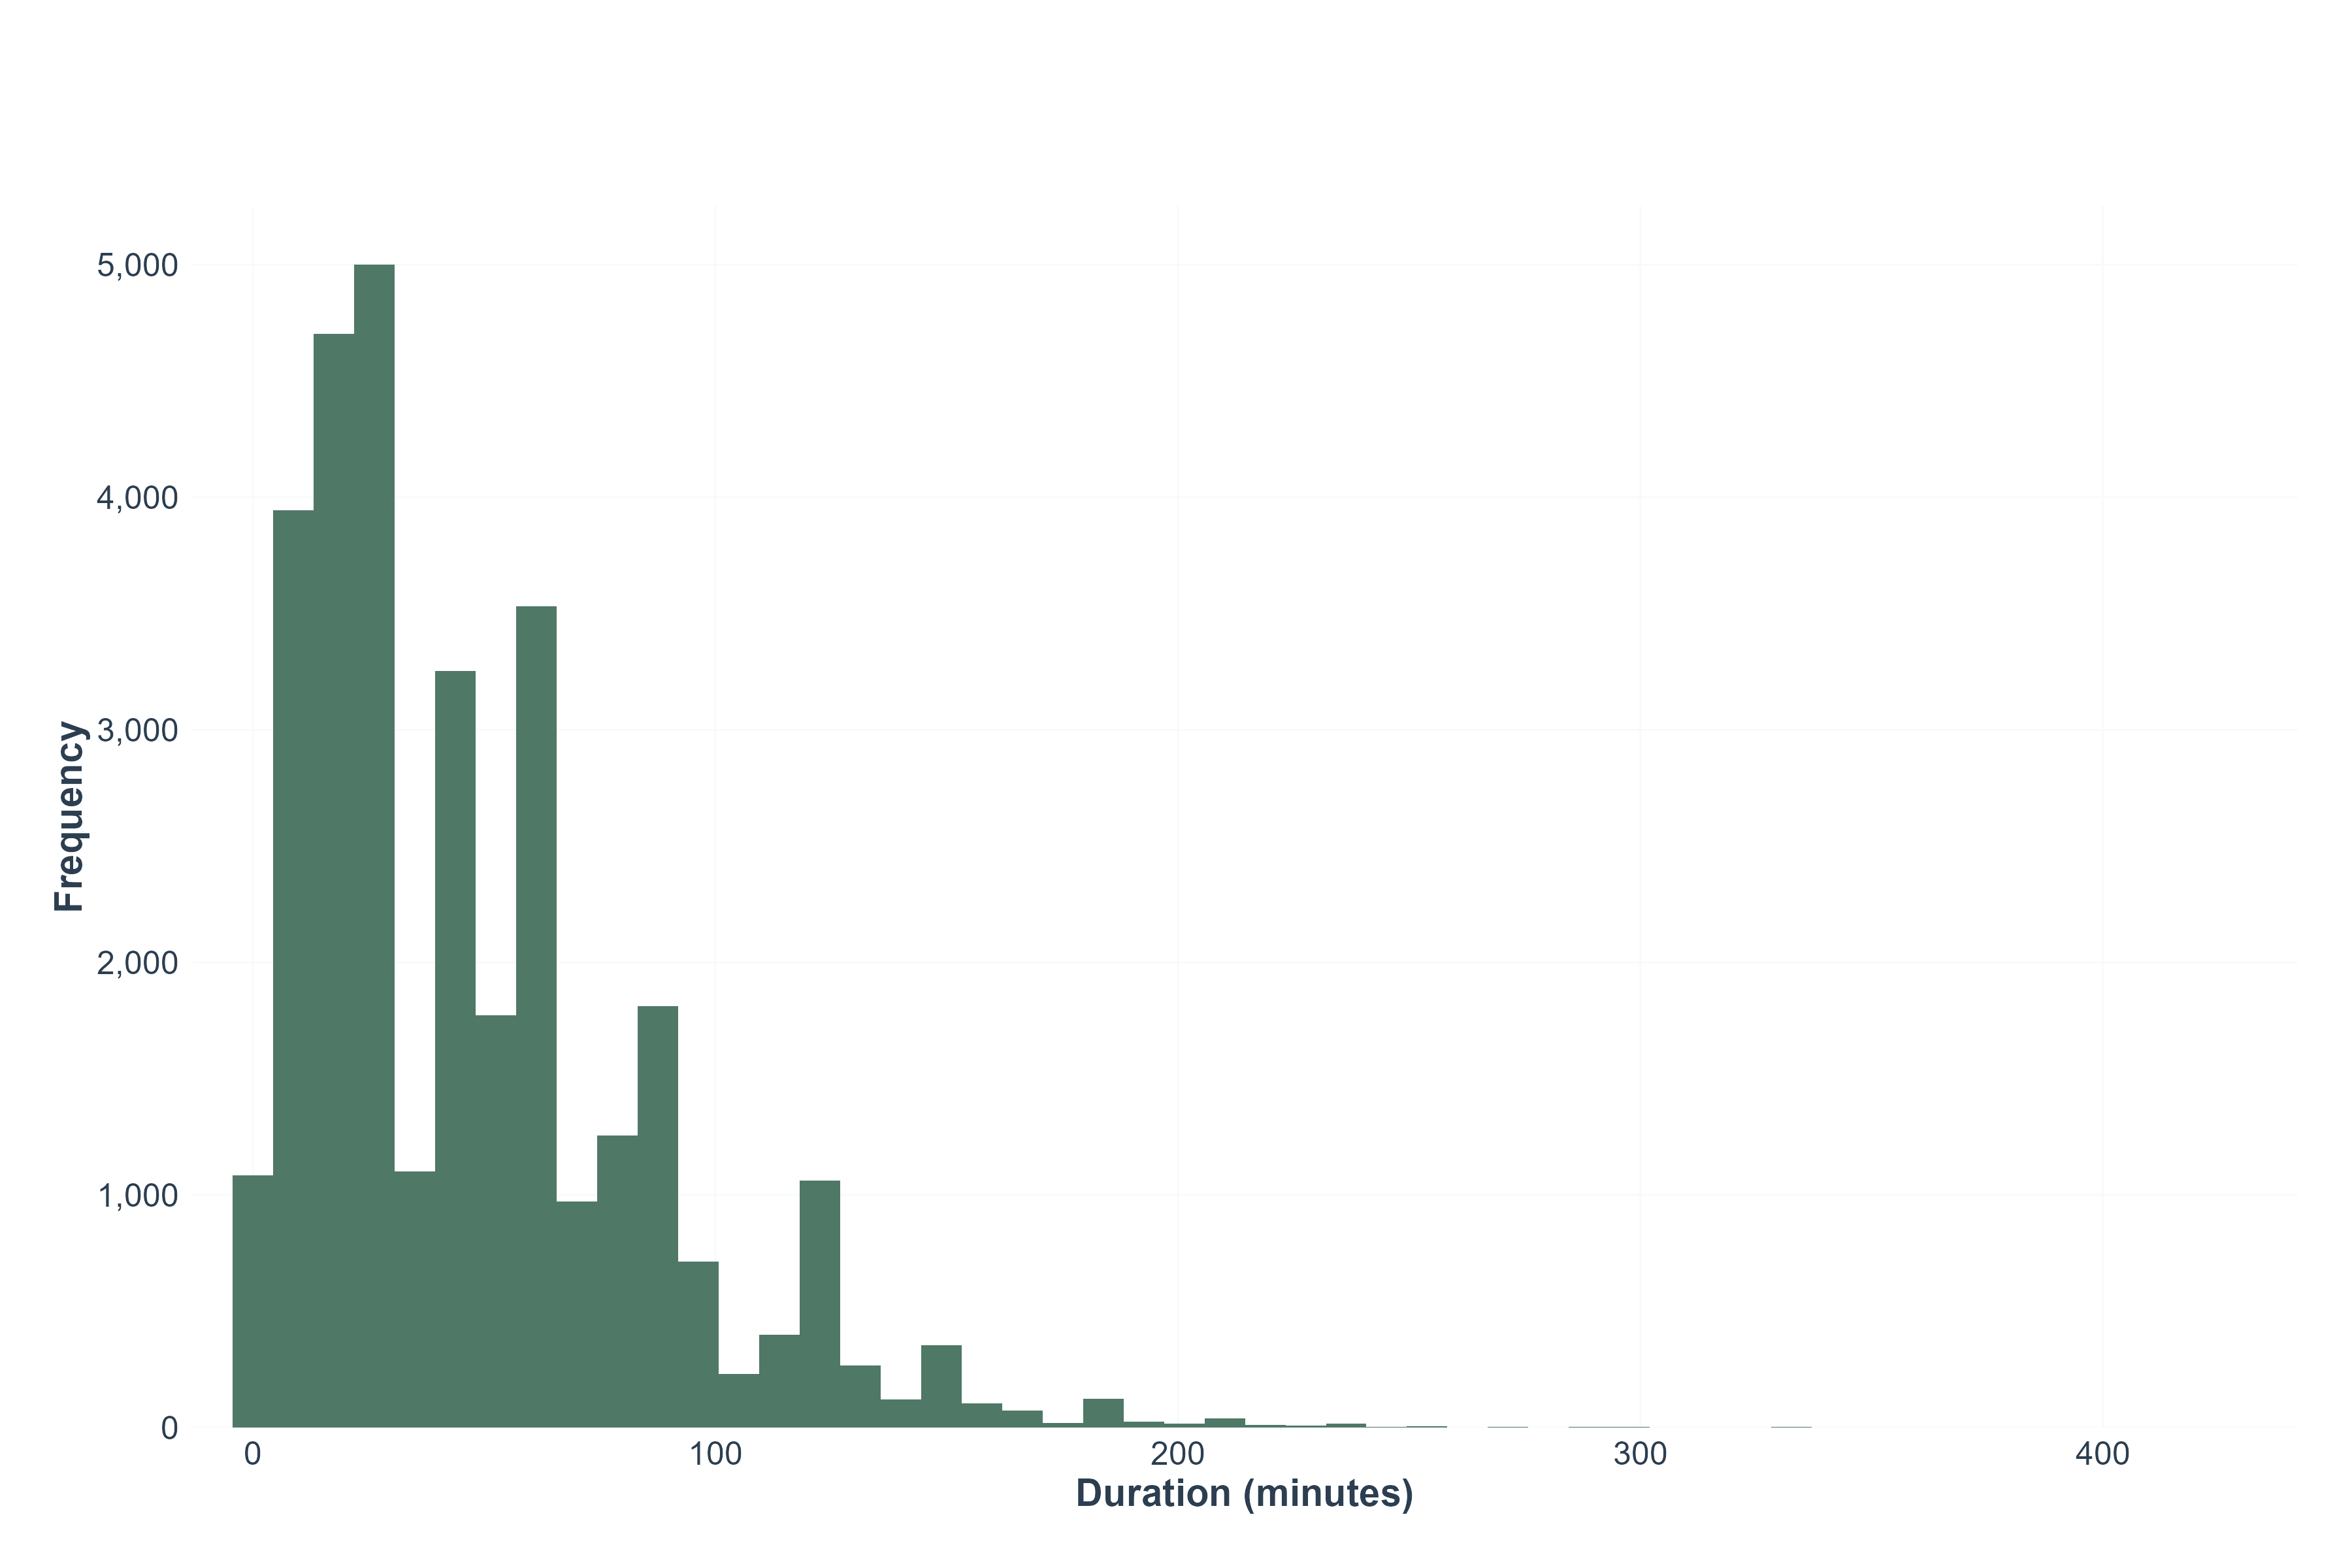
\includegraphics[width=0.8\textwidth]{../figures/duration_histogram.png}
    \caption{Histograms showing the distributions of rainfall (top), number of trips (middle), and trip durations (bottom) in the dataset.}
    \label{fig:hist}
\end{figure}

\begin{figure}[H]
    \centering
    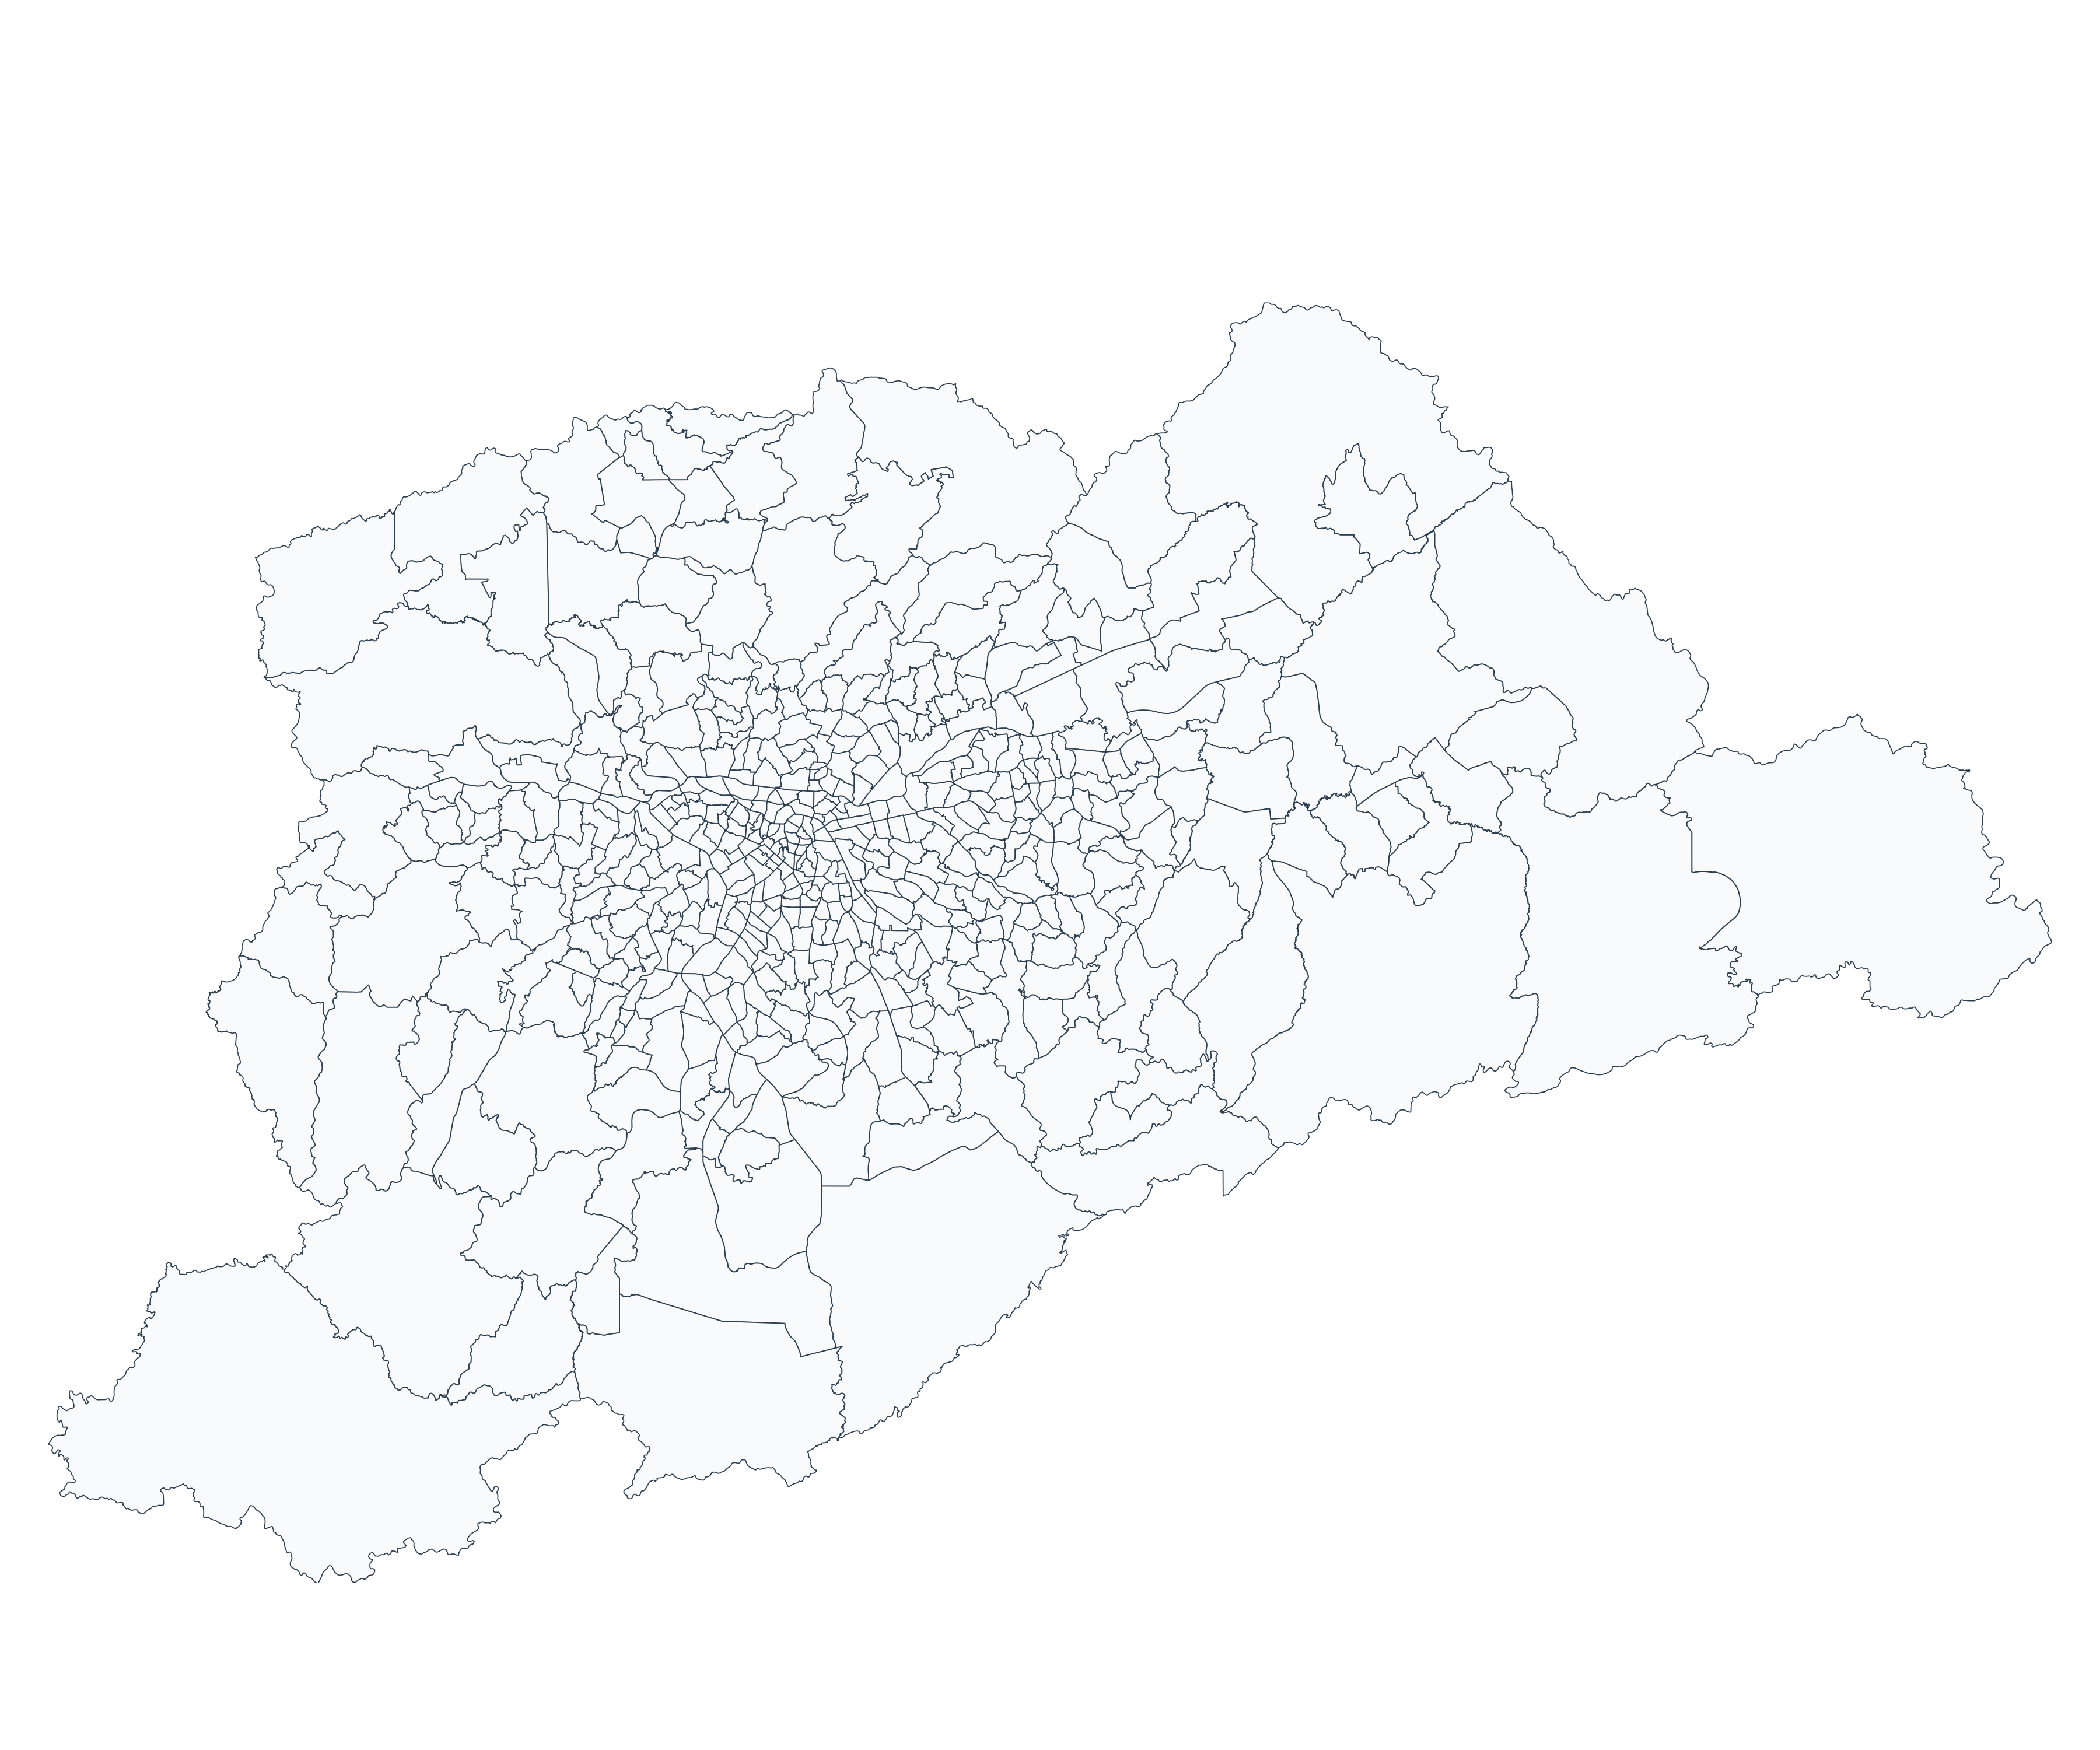
\includegraphics[width=0.8\textwidth]{../figures/rmsp_base.png}
    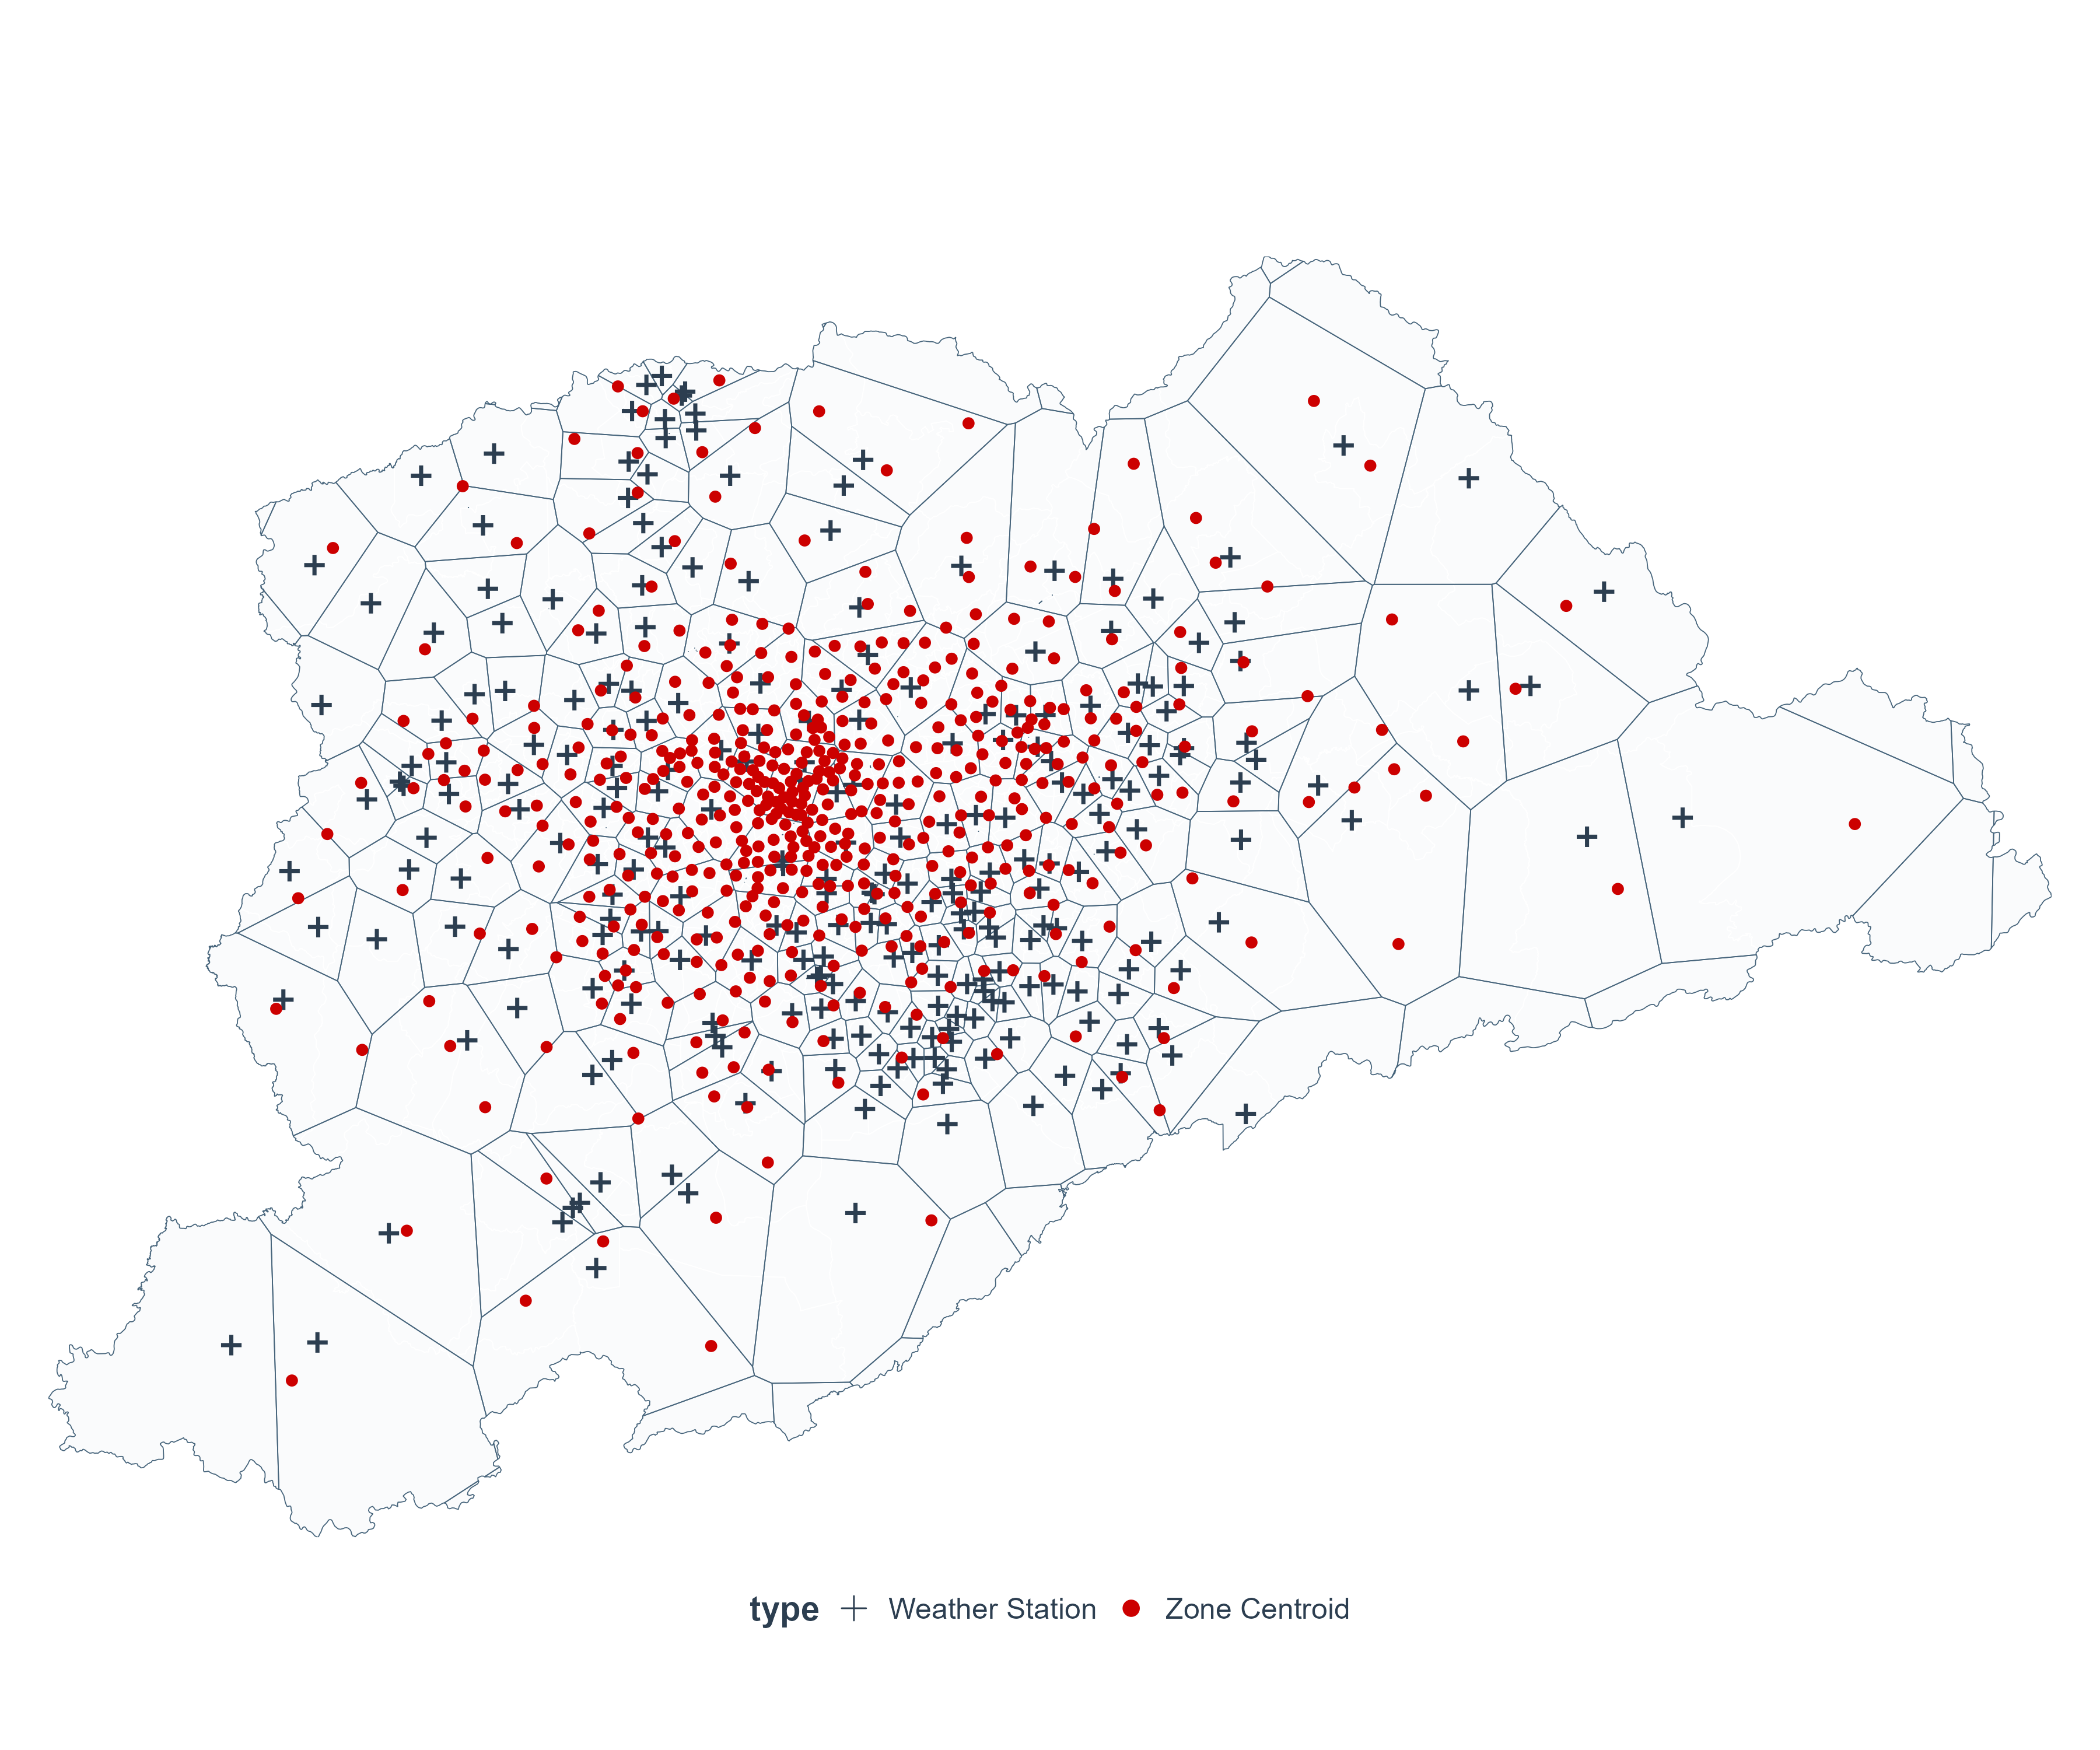
\includegraphics[width=0.8\textwidth]{../figures/rmsp_voronoi.png}
    \caption{Spatial representation of the RMSP region: (top) zone partitions, (bottom) Voronoi diagram illustrating spatial partitions based on centroid proximity to weather stations.}
    \label{fig:rmsp_voronoi}
\end{figure}


\label{tab:panel_a}
\begin{table}
\centering
\begin{talltblr}[         %% tabularray outer open
caption={Effect of Rainfall on Work Probability},
note{}={* p \num{< 0.1}, ** p \num{< 0.05}, *** p \num{< 0.01}},
note{ }={Sample consists of individuals regularly employed or do side gigs who worked on reference day. The dependent variable is a binary indicator equal to 1 if the individual worked on the reference day, 0 otherwise. Individual controls include age, gender dummy, education level, activity status, occupation, economic sector, and employment type. Zone fixed effects control for time-invariant spatial characteristics. Standard errors are heteroskedasticity-robust (HC1) and are shown in parentheses.},
]                     %% tabularray outer close
{                     %% tabularray inner open
colspec={Q[]Q[]Q[]Q[]Q[]Q[]},
column{2,3,4,5,6}={}{halign=c,},
column{1}={}{halign=l,},
hline{6}={1,2,3,4,5,6}{solid, black, 0.05em},
}                     %% tabularray inner close
\toprule
& Model 1 & Model 2 & Model 3 & Model 4 & Model 5 \\ \midrule %% TinyTableHeader
Rain Dummy (>0mm) & \num{-0.004} &  & \num{-0.004} & \num{-0.003} & \num{-0.001} \\
& (\num{0.003}) &  & (\num{0.004}) & (\num{0.004}) & (\num{0.004}) \\
Total Rainfall (mm) &  & \num{-0.000} & \num{0.000} & \num{-0.000} & \num{-0.000} \\
&  & (\num{0.000}) & (\num{0.000}) & (\num{0.000}) & (\num{0.000}) \\
Num.Obs. & \num{35488} & \num{35488} & \num{35488} & \num{35482} & \num{35482} \\
Individual Controls & No & No & No & Yes & Yes \\
Zone Fixed Effects & No & No & No & No & Yes \\
\bottomrule
\end{talltblr}

\end{table}

\label{tab:panel_b}
\begin{table}
\centering
\begin{talltblr}[         %% tabularray outer open
caption={Effect of Rainfall on Commute Duration},
note{}={* p \num{< 0.1}, ** p \num{< 0.05}, *** p \num{< 0.01}},
note{ }={Sample consists of individuals regularly employed or do side gigs who worked on reference day. The dependent variable is commute duration in minutes. Individual controls include age, gender dummy, education level, activity status, occupation, economic sector, and employment type. Zone fixed effects control for time-invariant spatial characteristics. Standard errors are heteroskedasticity-robust (HC1) and are shown in parentheses.},
]                     %% tabularray outer close
{                     %% tabularray inner open
colspec={Q[]Q[]Q[]Q[]Q[]Q[]},
column{2,3,4,5,6}={}{halign=c,},
column{1}={}{halign=l,},
hline{6}={1,2,3,4,5,6}{solid, black, 0.05em},
}                     %% tabularray inner close
\toprule
& Model 1 & Model 2 & Model 3 & Model 4 & Model 5 \\ \midrule %% TinyTableHeader
Rain Dummy (>0mm) & \num{-0.925}** &  & \num{-0.864}* & \num{-0.295} & \num{-0.144} \\
& (\num{0.436}) &  & (\num{0.488}) & (\num{0.473}) & (\num{0.483}) \\
Total Rainfall (mm) &  & \num{-0.035} & \num{-0.009} & \num{-0.023} & \num{0.019} \\
&  & (\num{0.031}) & (\num{0.034}) & (\num{0.033}) & (\num{0.034}) \\
Num.Obs. & \num{31715} & \num{31715} & \num{31715} & \num{31711} & \num{31711} \\
Individual Controls & No & No & No & Yes & Yes \\
Zone Fixed Effects & No & No & No & No & Yes \\
\bottomrule
\end{talltblr}

\end{table}
